\documentclass[12pt,a4paper]{article}

\usepackage[left=3.00cm, right=2.00cm, top=2.00cm, bottom=2.00cm]{geometry}
\usepackage{lmodern}
\usepackage[utf8]{inputenc}
\usepackage[brazil]{babel}

\usepackage{amssymb}
\usepackage{amsmath}
\usepackage{amsfonts}
\usepackage{pgfplots}
\pgfplotsset{compat=1.16}

\usepackage{graphicx}
\usepackage{indentfirst}
\usepackage{booktabs}
\usepackage{fancyvrb}
\usepackage{quoting}

\usepackage[linesnumbered,ruled,portuguese]{algorithm2e}

\usepackage[numbers]{natbib}
\usepackage{url}
\bibliographystyle{plainnat}

\usepackage{setspace}
\onehalfspacing

\author{Pablo Cecilio Oliveira\\
	Alexander Cristian}
\title{Algorítimos e Estrutura de Dados III\\
	Primeiro Trabalho Prático - Hipercampos}
\date{}

\begin{document}
\maketitle

\section{Introdução}

Na Ciência da Computação, o estudo de algorítimos para resolução de problemas geométricos é conhecido como Geometria Computacional. De forma geral, o objetivo deste ramo é resolver de maneira eficiente utilizando o menor número possível de operações sobre os elementos geométricos elementares.\cite{wiki:compgeo}

Dentre vários problemas geométricos temos o desafio conhecido como ''Hipercampos'', o qual pode ser visto em algumas maratonas de programação\cite{uri:hipercampo}. Neste trabalho é apresentado a solução para esse problema por meio de um algorítimo contido em um programa desenvolvido na linguagem em C.

\subsection{Hipercampos, especificação do problema}

No problema de Hipercampos, um plano cartesiano em $\mathbb{R}^2$ possui duas ''âncoras'', dois pontos $A$ e $B$, onde o eixo $Y$ das duas âncoras são iguais a zero, ou seja $A=(X_A ,0)$ e $B=(X_B , 0)$. Os valores do eixo $X$ das âncoras variam de $X_A$ até $X_B$, formando assim um segmento de reta horizontal, tal que $0 < X_A < X_B \leqslant 10^4$. (Figura \ref{fig:entrada})

\begin{figure}[!h]
	\caption{Exemplo de entrada para o problema.}
	\label{fig:entrada}
	\centering
	\begin{tikzpicture}[baseline]
	\pgfplotsset{width=8.5cm}
	\begin{axis}[
	title={},
	xmin=0, xmax=100,
	ymin=0, ymax=100,
	xtick={0,20,40,60,80,100},
	ytick={20,40,60,80,100},
	xmajorgrids=true,
	ymajorgrids=true,
	grid style=dashed,
	%legend style={draw=none},
	]
	
	\addplot[color=black,only marks,mark=square*,mark size=2pt]
	coordinates{(10,0)(50,0)};	
	
	\addplot[color=black,only marks,mark size=2pt]
	coordinates{
		(4,29)
		(15,15)
		(25,25)
		(35,14)
		(36,30)
		(45,6)
		(26,20)
		(21,10)
		(28,5)
		(40,24)
		(65,16)
		(80,75)
		%(50,62)
		(5,90)
		(60,50)
	};
	\legend{Âncoras}
	\end{axis}
	\end{tikzpicture}
	\footnotesize \\Fonte: autores
\end{figure}

Ao plano cartesiano também somam-se um conjunto $P$ de $N$ coordenadas $(X_i,Y_i)$, sendo que as $N$ coordenadas do Conjunto $P$ variam em seu total entre um e cem, $N (1 \leqslant N \leqslant 100)$. As coordenadas $(X_i,Y_i)$ podem variar entre $0$ até $10^4$, ou seja, $0 < X_i,Y_i \leqslant 10^4$.

O objetivo do problema de Hipercampos é ligar as coordenadas contidas em $P$ às âncoras $X_A$ e $X_B$, formando assim o máximo número de triângulos sem que esses se interceptem (Figura \ref{fig:solucionando}). E para esse proposito foi desenvolvido um algorítimo contido no programa apresentado neste trabalho.

\begin{figure}[!h]
	\caption{Hipercampos, solucionando.}
	\label{fig:solucionando}
	\begin{tikzpicture}[baseline]
	\pgfplotsset{width=8.3cm}
	\begin{axis}[
	title={},
	xmin=0, xmax=100,
	ymin=0, ymax=100,
	xtick={0,20,40,60,80,100},
	ytick={20,40,60,80,100},
	xmajorgrids=true,
	ymajorgrids=true,
	grid style=dashed,
	%legend style={draw=none},
	]	
	
	\addplot+[sharp plot,color=black,mark size=2pt]
	coordinates{
		(10,0)(4,29)(50,0)
		(10,0)(15,15)(50,0)
		(10,0)(25,25)(50,0)
		(10,0)(35,14)(50,0)
		(10,0)(36,30)(50,0)
		(10,0)(45,6)(50,0)
		(10,0)(26,20)(50,0)
		(10,0)(21,10)(50,0)
		(10,0)(28,5)(50,0)
		(10,0)(40,24)(50,0)
		(10,0)(65,16)(50,0)
		(10,0)(80,75)(50,0)
		%(10,0)(50,62)(50,0)
		(10,0)(5,90)(50,0)
		(10,0)(60,50)(50,0)
	};
	\end{axis}
	\end{tikzpicture}
	\begin{tikzpicture}[baseline]
	\pgfplotsset{width=8.3cm}
	\begin{axis}[
	title={},
	xmin=0, xmax=100,
	ymin=0, ymax=100,
	xtick={0,20,40,60,80,100},
	ytick={20,40,60,80,100},
	xmajorgrids=true,
	ymajorgrids=true,
	grid style=dashed,
	%legend style={draw=none},
	]	
	
	\addplot+[sharp plot,color=black,mark size=2pt]
	coordinates{
		(10,0)(28,5)(50,0)
		(10,0)(35,14)(50,0)
		(10,0)(40,24)(50,0)
		(10,0)(60,50)(50,0)
		(10,0)(80,75)(50,0)
	};
	\end{axis}
	\end{tikzpicture}
	\footnotesize \hphantom{space}Fonte: autores
\end{figure}

\subsection{Visão geral sobre o funcionamento do programa}

O programa desenvolvido recebe por parâmetro a entrada de um arquivo contendo em sua primeira linha um número $N$ total de coordenadas, e o valor para o eixo $X$ das âncoras $A$ e $B$ respectivamente. As linhas subsequentes a primeira correspondem às coordenadas das $N$ tuplas do conjunto $P$ a ser solucionado.

O algorítimo então processa esses dados retornando uma solução que pode ser verificada por meio de dois arquivos também gerados por um parâmetro: um contendo o número de triângulos possíveis e o outro em forma de uma imagem renderizada como ''gráfico vetorial escalável'' (Scalable Vector Graphics, ou ''.svg'')\footnote{Trata-se de uma linguagem XML para descrever de forma vetorial desenhos e gráficos bidimensionais.}. Um terceiro arquivo em ''.svg'' é gerado contendo a entrada original dos dados para referência.

O programa é executado no prompt de comando e recebe as passagens de parâmetro dos arquivos de entrada e saída:

\begin{figure}[!h]
\centering
\begin{BVerbatim}
$ ./hcamp -i [input] -o [output]
\end{BVerbatim}
\end{figure}

A entrada e solução renderizada pode ser vista no exemplo da Figura \ref{fig:inrend}.

\begin{figure}[!h]
	\caption{Entrada e saída renderizadas.}
	\vspace{5pt}
	\label{fig:inrend}
	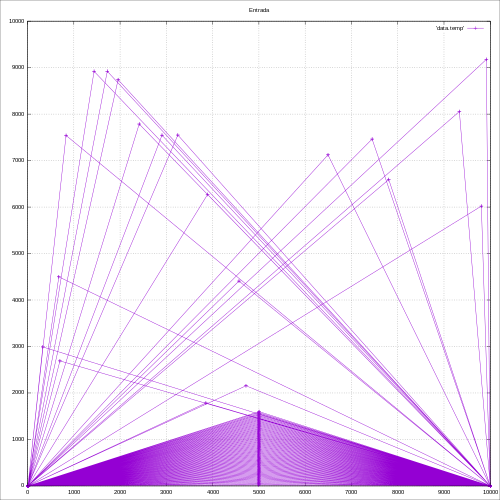
\includegraphics[width=75mm]{input.png}
	\hfill
	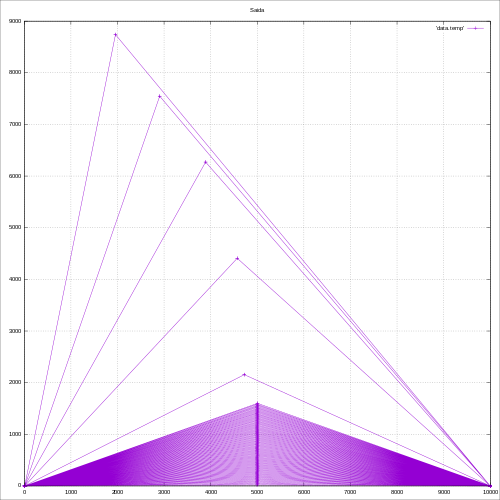
\includegraphics[width=75mm]{output.png}\\
	\footnotesize Fonte: via gnuplot com dados de entrada obtidos em uDebug.\cite{uri:vitor}
\end{figure}

\section{Implementação}

Inicialmente os dados contidos no arquivo de entrada são verificados e transferidos para uma lista simplesmente encadeada, esta limitada ao tamanho da memória principal disponível.

Após os dados estarem disponíveis na memória, uma função recursiva contendo um algorítimo para a solução determina entre todos os pontos do plano, qual ponto possui o maior numero de coordenadas dentro da área formada pelo ponto testado e suas duas âncoras. Este teste a principio tem como premissa o argumento em que o ponto com o maior número de coordenadas em sua área será aquele que terá o maior número de possibilidades de formações triangulares subsequentes.

O teste recursivo se repete sucessivamente para cada ponto interno em relação ao ponto inicialmente encontrado como sendo o de maior número de coordenadas (pontos $X_i,Y_i$), determinando o maior conjunto de elementos em relação ao conjunto anteriormente encontrado. O processo finaliza quando não existem mais coordenadas a serem encontradas.

A função que determina se uma coordenada está ou não dentro de uma área formada pelo ponto e suas duas ancoras é derivada do método do produto vetorial entre duas retas.\cite{jules:test} Este consiste em calcular a orientação do segmento de reta entre as âncoras e o ponto a ser testado com o ponto que forma um triangulo partindo das âncoras, determinando assim se o ponto testado está dentro da área formada pelo ponto de referência.

A equação que determina essa orientação é dada por:
\[(y2-y1)*(x3-x2) - (y3-y2)*(x2-x1)\]

Como o eixo $Y$ das âncoras são iguais a zero, a equação pode ser simplificada como: \[y2*(x3-x2) - (y3-y2)*(x2-x1)\]

Aplicando a equação entre os segmento de reta $\overline{PQ}$, sendo $P$ a âncora e $Q$ o ponto que forma o triângulo), com $\overline{PR}$ ($R$, ponto sendo testado), resulta no valor que determina a orientação da reta $\overline{PR}$ em relação a $\overline{PQ}$. No caso do resultado for maior que zero, a reta $\overline{PR}$ está no sentido horário a reta $\overline{PQ}$, caso seja menor do que zero, está está em sentido anti-horário à  $\overline{PQ}$.

A relação entre os segmentos de reta $\overline{PQ}$ e $\overline{PR}$ com as coordenadas respectivas às âncoras em $P$, determinam se um ponto está no sentido horário à $\overline{PQ_A}$ ou no sentido anti-horário à $\overline{PQ_B}$, definindo assim se este está dentro da área do triangulo formado entre as duas âncoras e o ponto Q.

A Figura \ref{fig:orientacao} demonstra esse o conceito.

\begin{figure}[!h]
	\caption{Determinando o ponto interno ao triângulo}
	\label{fig:orientacao}
	\begin{tikzpicture}[baseline]
	\pgfplotsset{width=8.3cm}
	\begin{axis}[
	title={},
	xmin=0, xmax=80,
	ymin=0, ymax=80,
	xtick={0,20,40,60,80,100},
	ytick={20,40,60,80,100},
	grid style=dashed,
	%legend style={draw=none},
	]	
	
	\addplot+[color=black,mark size=2pt]
	coordinates{
		(10,0)(40,75)
	};
	\addplot[color=red,mark size=2pt]
	coordinates{
		(10,0)(40,50)
	};
	
	\addplot[mark=*] coordinates {(40,50)} node[pin=310:{$PQR()>0$}]{};
	\addplot[mark=*] coordinates {(10,0)} node[pin=90:{$P$}]{};
	\addplot[mark=*] coordinates {(40,75)} node[pin=0:{$Q$}]{};
	\addplot[mark=*] coordinates {(40,50)} node[pin=0:{$R$}]{};
	
	\end{axis}
	\end{tikzpicture}
	\begin{tikzpicture}[baseline]
	\pgfplotsset{width=8.3cm}
	\begin{axis}[
	title={},
	xmin=0, xmax=80,
	ymin=0, ymax=80,
	xtick={0,20,40,60,80,100},
	ytick={20,40,60,80,100},
	grid style=dashed,
	%legend style={draw=none},
	]	
	
	\addplot+[color=black,mark size=2pt]
	coordinates{
		(70,0)(40,75)
	};
	\addplot[color=red,mark size=2pt]
	coordinates{
		(70,0)(40,50)
	};
	
	\addplot[mark=*] coordinates {(40,50)} node[pin=250:{$PQR()<0$}]{};
	\addplot[mark=*] coordinates {(70,0)} node[pin=90:{$P$}]{};
	\addplot[mark=*] coordinates {(40,75)} node[pin=180:{$Q$}]{};
	\addplot[mark=*] coordinates {(40,50)} node[pin=180:{$R$}]{};
	
	\end{axis}
	\end{tikzpicture}
	\footnotesize \hphantom{spac}Fonte: autores
\end{figure}

A implementação da solução se da então por meio de força bruta com o teste recursivo entre todas as coordenadas, determinando os triângulos que possuem sempre o maior numero de coordenadas em sua área.

O resultado para o número máximo de triângulos no plano que não se interceptam exceto em sua base é derivado do valor de triângulos que possuem o maior número de coordenadas em sua área.

A Tabela \ref{tab:funcoes} contém a lista das principais funções utilizadas no programa, uma descrição sucinta de suas finalidades e sua complexidade por tempo.

\pagebreak

\begin{table}[!htbp]
	\renewcommand{\arraystretch}{1.8}
	\caption{Funções do programa.}
	\label{tab:funcoes}
	\begin{tabular}{p{2.2cm} p{10cm} c}
		\toprule 
		Função & Finalidade & Complexidade* \\ 
		\midrule
		$debug()$ & Função que verifica a condição para retorno de possíveis bugs no programa. & $O(1)$ \\
		$create()$ & Inicializa uma lista simplesmente encadeada. & $O(1)$ \\
		$insere()$ & Insere os dados em uma lista encadeada. & $O(1)$ \\
		$printCJT()$ & Imprime uma lista encadeada. & $O(n)$ \\
		$sizeCJT()$ & Retorna o tamanho da lista encadeada. & $O(n)$ \\
		$dump()$ & Libera a memoria alocada pela lista encadeada criada. & $O(n)$ \\
		$isEmpty()$ & Verifica se uma lista encadeada está vazia. & $O(1)$ \\
		$openFILE()$ & Abre o arquivo solicitado e transfere os dados para uma lista encadeada. & $O(n)$ \\
		$saveFILE()$ & Salva a solução do problema em um arquivo. & $O(1)$ \\
		$chkFILE()$ & Verifica por possíveis erros de entrada em um arquivo. & $O(n)$ \\
		$showerro()$ & Retorna possíveis erros no arquivo de entrada. & $O(1)$ \\
		$ask()$ & Solicita a confirmação do usuário caso erros de entrada sejam encontrados. & $O(1)$ \\
		$cpyCJT()$ & Copia os dados de uma lista encadeada para outra lista encadeada. & $O(n)$ \\
		$PQR()$ & Algorítimo de orientação do ponto em relação a reta da ancora. & $O(1)$ \\
		$findMAX()$ & Função recursiva que determina o maior conjunto de pontos que se encontram dentro do triângulo formado pelas ancoras e um ponto $(x,y)$.  & $O(n)$ \\
		$soluciona()$ $solucao()$ & Funções de chamada e retorno para a execução do algorítimo & $O(1)$ \\
		$plotGraph()$ & PIPE para o gnuplot com a finalidade de renderizar os arquivos .svg contendo respectivamente, a entrada e saída da solução do problema.  & $O(n)$ \\ 
		\bottomrule
	\end{tabular}
	\footnotesize Fonte: autores\hfill *Complexidade por tempo.
\end{table}

\subsection{Análise de complexidade}

O algorítimo da função $findMAX()$ soluciona o problema operando recursivamente no conjunto de coordenadas, selecionando cada coordenada e comparando com todas as outras do conjunto. A cada comparação, o ponto de referencia as ancoras é testado em relação a todos os outros pontos do conjunto, caso os pontos verificados estejam dentro da área triangular formada pelo ponto de referencia, esses são inseridos em um conjunto auxiliar. 

Após todas as comparações terem sido feitas, esse conjunto auxiliar é comparado ao máximo de outros conjuntos previamente testados, e caso esse seja maior, passa a ser considerado como conjunto $MAX$.

O conjunto $MAX$ então é submetido a mesma função recursiva, que opera sobre os conjuntos \emph{máximos} encontrados até que não haja mais coordenadas a serem processadas. O pseudo-código é exemplificado abaixo como Algorítimo \ref{alg:findmax}.

\vspace{10pt}
\begin{algorithm}[H]
	\caption{findMAX()}
	\label{alg:findmax}
	\SetAlgoLined
	\Repita{até que todos os Pontos do Conjunto A tenham sido comparados}{
		\ParaTodo{ponto no Conjunto A}{
			Compare com todos os pontos do Conjunto A;\\
			\lSe{houverem pontos em sua área}{
				Insira em um Conjunto B
			}
			\lSe{B for Maior que o Conjunto anterior}{
				MAX = B
			}
		}
		Conjunto A = MAX;
	}
\end{algorithm}
\vspace{10pt}

O principal problema em identificar a complexidade é determinar qual é a probabilidade de cada ponto testado estar dentro da área de um ou mais triângulos. A cada comparação, a probabilidade de um conjunto ser ou não maior, ou o ponto pertencer ou não a esse conjunto pode ser respondida citando a questão abaixo:

Yang, stackoverflow.com, 2015: 

\begin{quoting}[rightmargin=0cm,leftmargin=4cm]
	\begin{singlespace}
	{\footnotesize  
	So I had to insert $N$ elements in random order into a size-N array, but I am not sure about the time complexity of the program.

	The program is basically:\\

	\begin{BVerbatim}
	for (i = 0 -> n-1) {
		index = random (0, n); // (n is exclusive)
		while (array[index] != null) {
			index = random (0, n);
		}
		array[index] = n;
	}
	\end{BVerbatim}

	}
	\end{singlespace}
	[...]
\end{quoting}

A resposta para o problema desta questão resolve o problema da probabilidade de comparações necessárias para determinar se um ponto pertence a um conjunto sucessivamente.

Pattison, stackoverflow.com, 2015:

\begin{quoting}[rightmargin=0cm,leftmargin=4cm]
	\begin{singlespace}
	{\footnotesize  
	First consider the inner loop. When do we expect to have our first success (find an open position) when there are $i$ values already in the array? For this we use the geometric distribution:
	\[Pr(X = k) = (1-p)^{k-1} p\]
	
	Where $p$ is the probability of success for an attempt. Here $p$ is the probability that the array index is not already filled. There are $i$ filled positions so $p = (1 - (i/n)) = ((n - i)/n)$.
	
	From the wiki, the expectation for the geometric distribution is $1/p = 1 / ((n-i)/n) = n/(n-i)$. Therefore, we should expect to make $(n / (n - i))$ attempts in the inner loop when there are $i$ items in the array.
	
	To fill the array, we insert a new value when the array has $i=0..n-1$ items in it. The amount of attempts we expect to make overall is the sum:
	
	\[ \begin{split}
	\sum_{i=0}^{n-1} \frac{n}{n-i}&= n * \sum_{i=0}^{n-1} (\frac{1}{(n-i)})\\
	&= n * (1/n + 1/(n-1) + ... + 1/1) \\
	&= n * (1/1 + ... + 1/(n-1) + 1/n) \\
	&= n * \sum_{i=1}^{n} \frac{1}{i}
	\end{split} \]
	
	Which is n times the $nth$ harmonic number and is approximately $\ln(n) + gamma$, where $gamma$ is a constant. So overall, the number of attempts is approximately $n * (\ln(n) + gamma)$, which is $O(n \log n)$. Remember that this is only the expectation and there is no true upper bound since the inner loop is random; it may never find an open spot.
	}
	\end{singlespace}
\end{quoting}

Considerando então o caso observado na citação, e derivando a mesma aplicação da solução ao problema do conjunto de probabilidades de comparações, podemos inicialmente concluir a função $f(n)$ em $findMAX()$, como sendo:

\[f(n)= n * n + 2n \log n\] 

\subsection{Tempos de computação}

Analisando as tomadas de tempo, observamos que o programa tem um comportamento $f(n) = n^2$. Para analisar os tempos da Tabela \ref{tab:tempos} e da Figura \ref{fig:tempos}, as funções $gettime$, $ru\_utime$ e $ru\_stime$ foram utilizadas.

A função $gettime$ atua como um cronômetro a partir de sua inicialização até a chamada para finalização da tomada do tempo a ser obtido, $ru\_utime$ representa o tempo usado pela CPU pelo usuário - o tempo, até um determinado ponto em que o processador levou para executar o código à nível de usuário (um modo restrito onde o código não tem acesso direto ao hardware subjacente) e $ru\_stime$ representa o tempo usado pela CPU pelo sistema - o tempo, até um determinado ponto em que o processador levou para executar o código à nível de kernel (um modo irrestrito onde o código tem acesso direto ao hardware subjacente).

\begin{table}[!h]
	\centering
	\caption{Tempos de execução em relação a entrada $n$.}
	\label{tab:tempos}
	\begin{tabular}{lrrr}
		\toprule 
		$n$ & $gettime()$ & $ru\_utime()$ & $ru\_stime()$ \\ 
		\midrule
		100 & 91751 $\mu$s & 9847 $\mu$s & 0 \\
		500 & 1418852 $\mu$s & 154276 $\mu$s & 3435 $\mu$s \\
		1000 & 2144396 $\mu$s & 559727 $\mu$s & 3290 $\mu$s \\
		2000 & 5350661 $\mu$s & 2s 246933 $\mu$s & 3324 $\mu$s \\
		4000 & 11219083 $\mu$s & 9s 167495 $\mu$s & 3333 $\mu$s \\
		8000 & 40450777 $\mu$s & 38s 906846 $\mu$s & 3324 $\mu$s \\
		16000 & 167955974 $\mu$s & 166s 90082 $\mu$s & 6662 $\mu$s \\
		\bottomrule
		\footnotesize Fonte: autores
	\end{tabular}
\end{table}

\begin{figure}[!h]
	\caption{Tempos de execução em relação a entrada $n$.}
	\label{fig:tempos}
	\begin{tikzpicture}
	\pgfplotsset{width=15cm}
	\begin{axis}[
	title={},
	xmin=100, xmax=16000,
	ymin=0, ymax=170,
	xlabel={Dados de entrada(n)},
	ylabel={Tempo de execução(s)},
	xtick={2000,4000,6000,8000,10000,12000,14000,16000},
	ytick={10,20,30,40,50,60,120,170},
	xmajorgrids=true,
	ymajorgrids=true,
	grid style=dashed,
	legend style={draw=none},
	]
	
	\addplot+[color=blue,mark size=2pt]
	coordinates{
		(100,0.091751)(500,1.418852)(1000,2.144396)(2000,5.350661)(4000,11.219083)
		(8000,40.450777)(16000,167.955974)
	};
	\legend{gettime(),$n^2$}
	\end{axis}
	\end{tikzpicture}
	\footnotesize \hphantom{spacessss}Fonte: autores
\end{figure}

\pagebreak

\section{Considerações finais}

Durante o desenvolvimento vários métodos foram testados com o objetivo de encontrar a maneira mais eficiente de encontrar a solução para o problema de Hipercampos. Foram considerados LCS\footnote{Longest common subsequence ou máxima subsequência crescente consiste em encontrar um subsequência de números, dada um sequência, na qual seus elementos estão ordenados  do menor para o maior, e a sequência é a mais longa possível.}, coordenadas baricêntricas\footnote{As Coordenadas Baricêntricas definem uma forma de representação de um ponto no espaço em função de outros pontos.} e outros métodos envolvendo o calculo da área formada pelos triângulos. Porém, não foi possível neste trabalho chegar a um resultado satisfatório quanto a aplicação desses métodos ao problema.

O uso de um algorítimo recursivo de força bruta foi o que mais se aproximou de um resultado preciso, mas mesmo esse método falhou em testes mais elaborados. A premissa de que o triângulo que contém com o maior número de coordenadas em sua área será aquele que terá o maior número de possibilidades de formações triangulares subsequentes, é incompleta, pois não considera a área dos triângulos formados. Esse erro pode ser verificado visualmente pela Figura \ref{fig:falsa}.

\begin{figure}[!h]
	\caption{Falha no algorítimo.}
	\label{fig:falsa}
	\begin{tikzpicture}[baseline]
	\pgfplotsset{width=8.3cm}
	\begin{axis}[
	title={},
	xmin=0, xmax=100,
	ymin=0, ymax=100,
	xtick={0,20,40,60,80,100},
	ytick={20,40,60,80,100},
	xmajorgrids=true,
	ymajorgrids=true,
	grid style=dashed,
	%legend style={draw=none},
	]
	
	\addplot+[sharp plot,color=black,mark size=2pt]
	coordinates{
		(10,0)(4,29)(40,0)
		(10,0)(15,15)(40,0)
		(10,0)(25,25)(40,0)
		(10,0)(35,14)(40,0)
		(10,0)(36,30)(40,0)
		(10,0)(45,6)(40,0)
		(10,0)(26,20)(40,0)
		(10,0)(21,10)(40,0)
		(10,0)(28,5)(40,0)
		(10,0)(40,24)(40,0)
		(10,0)(65,16)(40,0)
		(10,0)(80,75)(40,0)
		(10,0)(50,62)(40,0)
		(10,0)(5,90)(40,0)
		(10,0)(60,50)(40,0)
	};
	\end{axis}
	\end{tikzpicture}
	\begin{tikzpicture}[baseline]
	\pgfplotsset{width=8.3cm}
	\begin{axis}[
	title={},
	xmin=0, xmax=100,
	ymin=0, ymax=100,
	xtick={0,20,40,60,80,100},
	ytick={20,40,60,80,100},
	xmajorgrids=true,
	ymajorgrids=true,
	grid style=dashed,
	%legend style={draw=none},
	]	
	
	\addplot+[sharp plot,color=blue,mark size=2pt]
	coordinates{
		(10,0)(28,5)(40,0)
		(10,0)(35,14)(40,0)
		(10,0)(40,24)(40,0)
		(10,0)(60,50)(40,0)
		(10,0)(80,75)(40,0)
	};

	\addplot+[sharp plot,color=red,mark size=2pt]
	coordinates{
		(10,0)(28,5)(40,0)
		(10,0)(35,14)(40,0)
		(10,0)(36,30)(40,0)
		(10,0)(50,62)(40,0)
	};
	\legend{Solução correta,Algoritimo}
	\end{axis}
	\end{tikzpicture}
	\begin{tikzpicture}[baseline]
	\pgfplotsset{width=8.3cm}
	\begin{axis}[
	title={},
	xmin=0, xmax=100,
	ymin=0, ymax=100,
	xtick={0,20,40,60,80,100},
	ytick={20,40,60,80,100},
	xmajorgrids=true,
	ymajorgrids=true,
	grid style=dashed,
	%legend style={draw=none},
	]	
	
	\addplot+[sharp plot,color=red,mark size=2pt]
	coordinates{
		(10,0)(28,5)(40,0)
		(10,0)(35,14)(40,0)
		(10,0)(36,30)(40,0)
		(10,0)(50,62)(40,0)
	};
	\end{axis}
	\end{tikzpicture}
	\begin{tikzpicture}[baseline]
	\pgfplotsset{width=8.3cm}
	\begin{axis}[
	title={},
	xmin=0, xmax=100,
	ymin=0, ymax=100,
	xtick={0,20,40,60,80,100},
	ytick={20,40,60,80,100},
	xmajorgrids=true,
	ymajorgrids=true,
	grid style=dashed,
	%legend style={draw=none},
	]	
	
	\addplot+[sharp plot,color=blue,mark size=2pt]
	coordinates{
		(10,0)(28,5)(40,0)
		(10,0)(35,14)(40,0)
		(10,0)(40,24)(40,0)
		(10,0)(60,50)(40,0)
		(10,0)(80,75)(40,0)
	};
	\end{axis}
	\end{tikzpicture}
\end{figure}

O algorítimo sempre escolhe o triangulo com o maior número de coordenadas em sua área, não considerando que essas possam ser eliminadas em teste subsequentes. Quanto maior a área do triangulo testado, maior sera a possibilidade de erros. E embora o programa cumpra a função de determinar um número de triângulos que não se interceptam, esse não é preciso quanto ao valor máximo que pode ser obtido.

Uma solução alternativa envolvendo o conceito de ''dividir para conquistar'' seria utilizar como entradas para um algorítimo, duas arvores binarias, cada uma delas conteria como raiz uma das ancoras e como filhos as coordenadas do arquivo de entrada. O algorítimo então testaria colisões, verificando se a reta formada a partir de um ponto até às âncoras é concorrente à alguma das retas encontradas em uma das duas árvores binarias. Porém não se chegou a um algorítimo eficaz que pudesse decidir entre um numero de colisões iguais.

\begin{flushleft}
	\nocite{*}
	\bibliography{tp_hcamp}
	\vfill
	O histórico do desenvolvimento desse trabalho se encontra online em:\\ \url{https://github.com/Durfan/ufsj-aeds3-tp1}.
\end{flushleft}

\end{document}
